\documentclass{article}
% generated by Madoko, version 1.0.0-rc5
%mdk-data-line={1}


\usepackage[heading-base={2},section-num={False},bib-label={True}]{madoko2}


\begin{document}



%mdk-data-line={7}
\mdxtitleblockstart{}
%mdk-data-line={7}
\mdxtitle{\mdline{7}Optimization of a DNN program on the CPU+MIC}%mdk
\mdxauthorstart{}
%mdk-data-line={12}
\mdxauthorname{\mdline{12}University of Electronic Secience and Technology of China}%mdk
\mdxauthorend\mdtitleauthorrunning{}{}\mdxtitleblockend%mdk

%mdk-data-line={9}
\begin{abstract}%mdk

%mdk-data-line={10}
\noindent\mdline{10}This article is a part of competition proposal of ASC, Asia Supercomputer Student Challenge. We analysis the \mdline{10}\mdcode{DNN}\mdline{10} program, put forward different optimization methods and point their pros and cons. In the end we talk about our shortcomings.%mdk
%mdk
\end{abstract}%mdk

%mdk-data-line={12}
\section{\mdline{12}1.\hspace*{0.5em}\mdline{12}Introduction}\label{sec-introduction}%mdk%mdk

%mdk-data-line={13}
\noindent\mdline{13}In the section a program based on a standalone hybrid CPU+MIC platform called \mdline{13}\mdcode{DNN(deep~neural~network)}\mdline{13} should be parallelized to obtain better performance. There is detailed information about hardware in Figure 1, software configuration in Figure 2.%mdk

%mdk-data-line={14}
\begin{figure}[tbp]%mdk
\begin{mdcenter}%mdk

%mdk-data-line={16}
\noindent\mdline{16}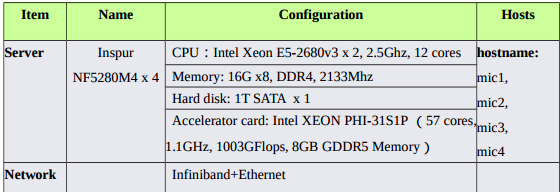
\includegraphics[keepaspectratio=true,width=\dimmin{}{\dimwidth{0.90}}]{images/2016-02-18-23-01-13-}{}\mdline{16}%mdk

%mdk-data-line={19}
\mdhr{}%mdk

%mdk-data-line={20}
\noindent\mdline{20}\mdcaption{\textbf{Figure~\mdcaptionlabel{1}.}~\mdcaptiontext{Hardware configuration}}%mdk
%mdk
\end{mdcenter}\label{fig-myfigure}%mdk
%mdk
\end{figure}%mdk

%mdk-data-line={21}
\begin{figure}[tbp]%mdk
\begin{mdcenter}%mdk

%mdk-data-line={22}
\noindent\mdline{22}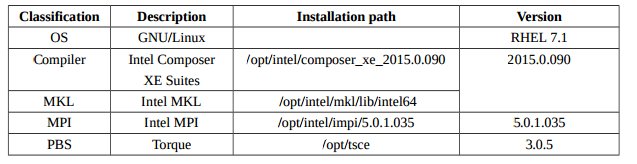
\includegraphics[keepaspectratio=true,width=\dimmin{}{\dimwidth{0.90}}]{images/2016-02-18-23-13-11-}{}\mdline{22}%mdk

%mdk-data-line={25}
\mdhr{}%mdk

%mdk-data-line={26}
\noindent\mdline{26}\mdcaption{\textbf{Figure~\mdcaptionlabel{2}.}~\mdcaptiontext{Software configuration}}%mdk
%mdk
\end{mdcenter}\label{fig-myfigure}%mdk
%mdk
\end{figure}%mdk

%mdk-data-line={27}
\section{\mdline{27}2.\hspace*{0.5em}\mdline{27}Analysis of the serial program}\label{sec-analysis-of-the-serial-program}%mdk%mdk

%mdk-data-line={28}
\noindent\mdline{28}First, a call graph(Figure 3.) is generated by using \mdline{28}\mdcode{Google~perfools}\mdline{28},
 a open source performance profiler, to have a glance though it. Every square represents a function, and the bigger square is, the more time corresponding function cost.%mdk

%mdk-data-line={31}
\begin{figure}[tbp]%mdk
\begin{mdcenter}%mdk

%mdk-data-line={32}
\noindent\mdline{32}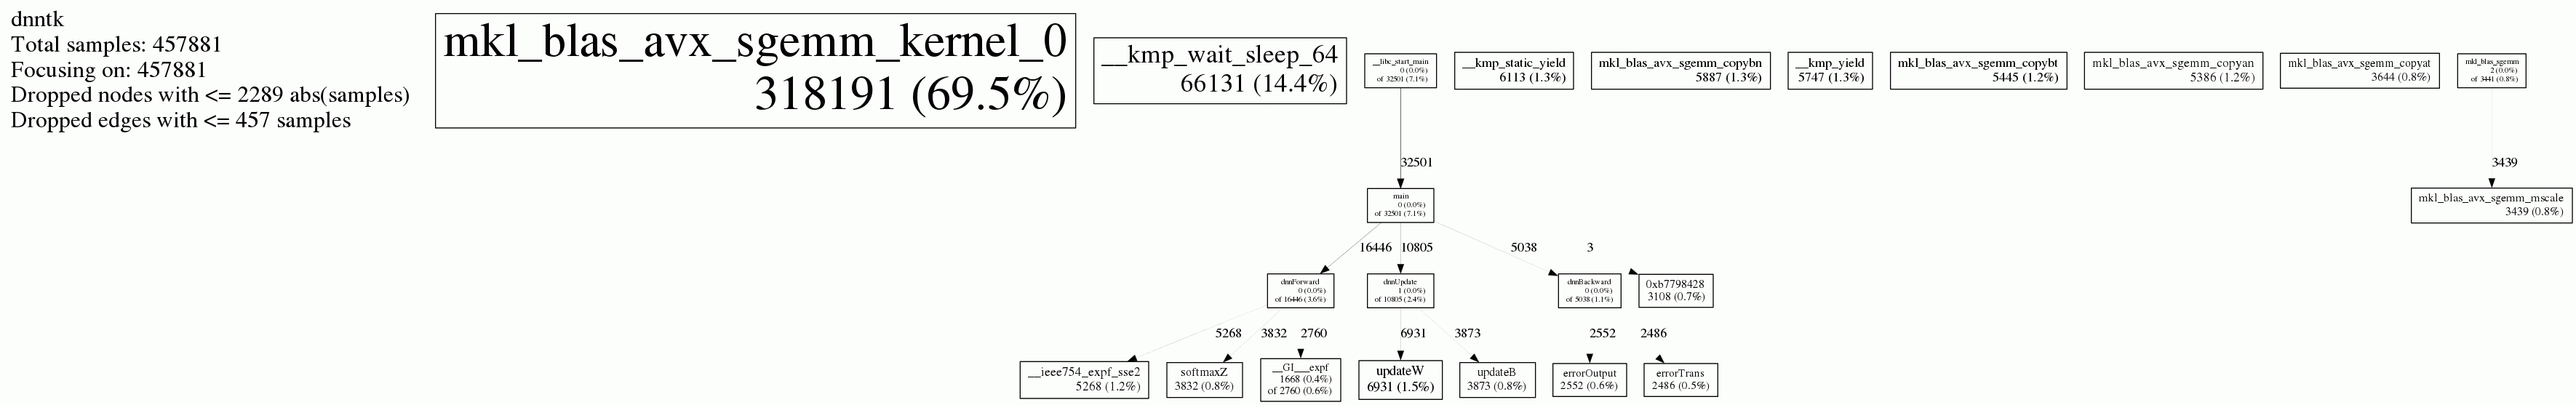
\includegraphics[keepaspectratio=true,width=\dimmin{}{\dimwidth{0.90}}]{images/100001994364201}{}\mdline{32}%mdk

%mdk-data-line={35}
\mdhr{}%mdk

%mdk-data-line={36}
\noindent\mdline{36}\mdcaption{\textbf{Figure~\mdcaptionlabel{3}.}~\mdcaptiontext{Google Perfools results}}%mdk
%mdk
\end{mdcenter}\label{fig-myfigure}%mdk
%mdk
\end{figure}%mdk

%mdk-data-line={38}
\mdline{38}Obviously, the hot spot is something about \mdline{38}\mdcode{MKL}\mdline{38}. After googling
and searching Intel document we know that MKL provides \mdline{39}\mdcode{BLAS~routinues}\mdline{39}, which includes a serial function named \mdline{39}\mdcode{cblas\_?gemm}\mdline{39}
to compute a matrix-matrix product with general matrices.%mdk

%mdk-data-line={42}
\mdline{42}But giving that MKL function is well-optimized, we search for all position where \mdline{42}\mdcode{cblas\_*gemm}\mdline{42} is called. Results show the usage of \mdline{42}\mdcode{cblas\_*gemm}\mdline{42} appear in file \mdline{42}\mdcode{dnn\_func.cpp}\mdline{42}, more specifically, in three function:%mdk

%mdk-data-line={44}
\begin{itemize}[noitemsep,topsep=\mdcompacttopsep]%mdk

%mdk-data-line={44}
\item\mdline{44}\mdcode{\preindent{1}extern~"C"~int~dnnForward(NodeArg~\&nodeArg)}\mdline{44}%mdk

%mdk-data-line={45}
\item\mdline{45}\mdcode{\preindent{1}extern~"C"~int~dnnBackward(NodeArg~\&nodeArg)}\mdline{45}%mdk

%mdk-data-line={46}
\item\mdline{46}\mdcode{\preindent{1}extern~"C"~int~dnnUpdate(NodeArg~\&nodeArg)}\mdline{46}%mdk
%mdk
\end{itemize}%mdk

%mdk-data-line={48}
\noindent\mdline{48}They call \mdline{48}\mdcode{MKL}\mdline{48} function \mdline{48}\mdcode{cblas\_sgemm}\mdline{48} many times by \mdline{48}\mdcode{for~loop}\mdline{48} and 
cost almost 90\% of all CPU time. So we guess that those function
 is what we may optimize, aka, hotspots.
The report(see Figure 4.) showed by\mdline{51}\mdcode{Intel~VTune}\mdline{51}, another profiler, proves our guess.%mdk

%mdk-data-line={53}
\begin{figure}[tbp]%mdk
\begin{mdcenter}%mdk

%mdk-data-line={54}
\noindent\mdline{54}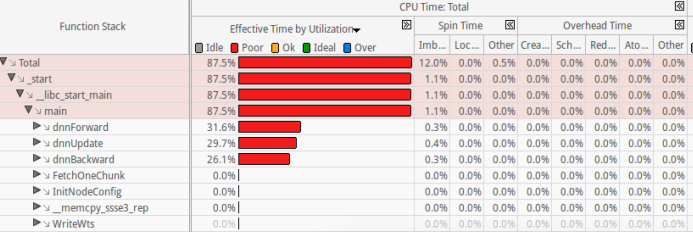
\includegraphics[keepaspectratio=true,width=\dimmin{}{\dimwidth{0.90}}]{images/2016-02-19-10-36-25-}{}\mdline{54}%mdk

%mdk-data-line={56}
\mdhr{}%mdk

%mdk-data-line={57}
\noindent\mdline{57}\mdcaption{\textbf{Figure~\mdcaptionlabel{4}.}~\mdcaptiontext{Intel VTune top-down tree}}%mdk
%mdk
\end{mdcenter}\label{fig-myfigure}%mdk
%mdk
\end{figure}%mdk

%mdk-data-line={58}
\mdline{58}After a skim through the source code, a clear structure 
about the program is established. To simplify describe, original program could be rewritten in pseudocode:%mdk
\begin{mdpre}%mdk
\noindent{\mdcolor{purple}1}.~{\mdcolor{teal}GetInitFileConfig}(cpuArg)\\
{\mdcolor{purple}2}.~{\mdcolor{teal}While}~{\mdcolor{teal}FetchOneChunk}(cpuArg,~onChunk)~{\mdcolor{navy}do}:\\
{\mdcolor{purple}3}.~~~~~~~{\mdcolor{teal}While}~{\mdcolor{teal}FetchOneBunch}(oneChunk,~nodeArg)~{\mdcolor{navy}do}:\\
{\mdcolor{purple}4}.~~~~~~~~~~~~dnnForward(nodeArg)\\
{\mdcolor{purple}5}.~~~~~~~~~~~~dnnBackward(nodeArg)\\
{\mdcolor{purple}6}.~~~~~~~~~~~~dnnUpate(nodeArg)\\
{\mdcolor{purple}7}.~{\mdcolor{teal}WriteWts}(nodeArg,~cpuArg)\\
{\mdcolor{purple}8}.~{\mdcolor{teal}UninitProgramConfig}(cpuArg)\\
%mdk
\end{mdpre}\noindent\mdline{73}There are two nested loop before \mdline{73}\mdcode{dnn*()}\mdline{73} processing function, and 
in each of those processing function many matrix-matrix product are
executed. Whether those hotspots could be parallelized or not depends
on data scale, dependency and so on. In the rest of this article some
methods are considered and weighed their pros and cons.

%mdk-data-line={79}
\section{\mdline{79}3.\hspace*{0.5em}\mdline{79}Fine grain parallelism}\label{sec-fine-grain-parallelism}%mdk%mdk

%mdk-data-line={80}
\noindent\mdline{80}In fine grain parallelism a thorough check is necessary. It\mdline{80}'\mdline{80}s better to look through the whole top-down tree rendered by \mdline{80}\mdcode{Intel~VTune}\mdline{80} and to find out performance-critical loop. Attention should be given to the \mdline{80}\mdcode{dnn*}\mdline{80} function series.%mdk

%mdk-data-line={82}
\mdline{82}In function \mdline{82}\mdcode{dnnForward}\mdline{82}, it\mdline{82}'\mdline{82}s easy to observe there is a \mdline{82}\mdcode{for~loop}\mdline{82} calling \mdline{82}\mdcode{cblas\_sgemm}\mdline{82}, which nearly cost all CPU time consumed by this function. But there is some detail should be consider in before optimization.%mdk

%mdk-data-line={84}
\subsection{\mdline{84}3.1.\hspace*{0.5em}\mdline{84}Matrix size}\label{sec-matrix-size}%mdk%mdk

%mdk-data-line={86}
\noindent\mdline{86}All \mdline{86}\mdcode{cblas\_sgemm}\mdline{86} is called like this:%mdk
\begin{mdpre}%mdk
\noindent~~cblas\_sgemm({\mdcolor{teal}CblasRowMajor},~{\mdcolor{teal}CblasNoTrans},~{\mdcolor{teal}CblasNoTrans},\textbackslash{}\\
~~~~~~~~numN,~numA[i],~numA[i-{\mdcolor{purple}1}],~\textbackslash{}\\
~~~~~~~~one,~d\_Y[i-{\mdcolor{purple}1}],~numA[i-{\mdcolor{purple}1}],~d\_W[i],~numA[i],~one,~d\_Y[i],~numA[i]);%mdk
\end{mdpre}\noindent\mdline{92}The arguments \mdline{92}\mdcode{numN}\mdline{92}, \mdline{92}\mdcode{numA[i]}\mdline{92}, \mdline{92}\mdcode{numA[i-1]}\mdline{92} indicating the size of the matrices:

%mdk-data-line={94}
\begin{itemize}[noitemsep,topsep=\mdcompacttopsep]%mdk

%mdk-data-line={94}
\item\mdline{94}\mdcode{d\_Y[i-1]}\mdline{94} is a \mdline{94}\mdcode{numN}\mdline{94} row by \mdline{94}\mdcode{numA[i]}\mdline{94} column matrix;%mdk

%mdk-data-line={95}
\item\mdline{95}\mdcode{d\_W[i]}\mdline{95} is a \mdline{95}\mdcode{numN}\mdline{95} row by \mdline{95}\mdcode{numA[i-1]}\mdline{95} column matrix;%mdk

%mdk-data-line={96}
\item\mdline{96}\mdcode{d\_Y[i]}\mdline{96} is a \mdline{96}\mdcode{numA[i-1]}\mdline{96} row by \mdline{96}\mdcode{numA[i]}\mdline{96} column matrix.%mdk
%mdk
\end{itemize}%mdk

%mdk-data-line={98}
\noindent\mdline{98}As we known the bigger matrix size is, the higher degree of \mdline{98}\mdcode{MKL}\mdline{98} parallelism is. But in the \mdline{98}\mdcode{DNN}\mdline{98} program, the size of matrix is decided by \mdline{98}\mdcode{bunchSize}\mdline{98}, a constant integer (\mdline{98}\ensuremath{\approx}\mdline{98}1024), and element (\mdline{98}\ensuremath{\approx}\mdline{98}1024) of \mdline{98}\mdcode{dnnLayerArr}\mdline{98}, a constant integer array. The two integers are configured by specified file, and we are not allowed to modify it. For this reason there are no sufficiently large matrix to enable \mdline{98}\mdcode{auto~offload~model}\mdline{98} to speed up \mdline{98}\mdcode{DNN}\mdline{98}.\mdline{98}[\mdcite{mkl-mic}{1}]\mdline{98}%mdk

%mdk-data-line={100}
\subsection{\mdline{100}3.2.\hspace*{0.5em}\mdline{100}Cycles index}\label{sec-cycles-index}%mdk%mdk

%mdk-data-line={101}
\noindent\mdline{101}In the \mdline{101}\mdcode{dnn*}\mdline{101} series every loop call \mdline{101}\mdcode{cblas\_sgemm}\mdline{101} \mdline{101}\mdcode{numN}\mdline{101}(\mdline{101}\ensuremath{\approx}\mdline{101}7) times, which indicates the length of \mdline{101}\mdcode{dnnLayerArr}\mdline{101}. It\mdline{101}'\mdline{101}s regretful that the value cannot be modified by us. Giving the multi-core of cluster it\mdline{101}'\mdline{101}s not wise to parallelize those loops.%mdk

%mdk-data-line={103}
\subsection{\mdline{103}3.3.\hspace*{0.5em}\mdline{103}Optimization method}\label{sec-optimization-method}%mdk%mdk

%mdk-data-line={104}
\subsubsection{\mdline{104}3.3.1.\hspace*{0.5em}\mdline{104}Serial \mdline{104}\mdcode{MKL}\mdline{104} function\mdline{104} \mdline{104}+}\label{sec-serial-mkl-function-}%mdk%mdk

%mdk-data-line={106}
\section{\mdline{106}4.\hspace*{0.5em}\mdline{106}Coarse grain parallelism}\label{sec-coarse-grain-parallelism}%mdk%mdk

%mdk-data-line={107}
\noindent\mdline{107}To implenment coarse grain parallelism we hope that each thread/process finish large subcomponents. To achieve this goal \mdline{107}\mdcode{DNN}\mdline{107} program should be divided into (mostly) independent and similar proportions, and every proportion should be as large as possible.%mdk

%mdk-data-line={109;out/document-bib.bbl.mdk:1}
%mdk-data-line={109;out/document-bib.bbl.mdk:2}
\mdsetrefname{References}%mdk
{\mdbibindent{0}%mdk
\begin{thebibliography}{1}%mdk
\label{sec-bibliography}%mdk

%mdk-data-line={reference.bib:1}
\bibitem{mkl-mic}Noah Clemons. \emph{Intel MKL Resource}. Intel, https://software.intel.com/en-us/articles/recommendations-to-choose-the-right-mkl-usage-model-for-xeon-phi. Mar. 2013.\label{mkl-mic}%mdk%mdk
\par%mdk
\end{thebibliography}}%mdk%mdk%mdk


\end{document}
